\chapter{Machine Learning}

The term machine learning was firstly coined in 1959 by Arthur Samuel. He described machine learning as: "the field of study that gives computers the ability to learn without being explicitly programmed."\cite{machine-learning-samuel}.

Tom M. Mitchell proposed a new formal definition in 1997\cite{machine-learning-mitchell}, which is:
\begin{definition}
A computer program is said to learn from experience $E$ with respect to some class of tasks $T$ and performance measure $P$, if its performance at tasks in $T$, as measured by $P$, improves with experience $E$.
\end{definition} 

Mitchell also describes an example where a computer program that learns to play chess improves its performance $P$ by gaining experience $E$ from games played against itself. Performance $P$ is measured as the ability to win in a class of tasks $T$, which in this example are the tasks of playing checkers.

\subsection*{A checkers learning problem:}

\begin{itemize}
    \item Task $T$: playing checkers
    \item Performace measure $P$: percent of games won againts humans or other programs
    \item Training experience $E$: percent of games won againts itself
\end{itemize}


Mitchell continues that all learning problems can be specified in this way, such as learning to recognise handwritten words, or learning to drive a robotic automobile autonomously.

\subsection*{A handwritten recognition learning problem:}

\begin{itemize}
    \item Task $T$: recognising and classifying handwritten words in a picture
    \item Performace measure $P$: percent of correctly recognised words
    \item Training experience $E$: a dataset of handwritten words with correct recognition
\end{itemize}

\subsection*{A robot driving learning problem:}

\begin{itemize}
    \item Task $T$: driving on a highway using cameras
    \item Performace measure $P$: average distance travelled before an error occurs
    \item Training experience $E$: a recorded video of a human driver as a sequence of images and steering commands
\end{itemize}

\section{Approaches}

Traditionally, all machine learning tasks can be divided into three broad categories according to the type of feedback provided to the learning system. These are supervised learning, unsupervised learning, and reinforcement learning\cite{ml-types1,ml-types2}.

Reinforcement learning is not described at all in this thesis, as reinforcement learning is not suitable for any type of machine learning problem addressed in the practical part of the thesis.

\begin{figure}[ht]
    \centering
    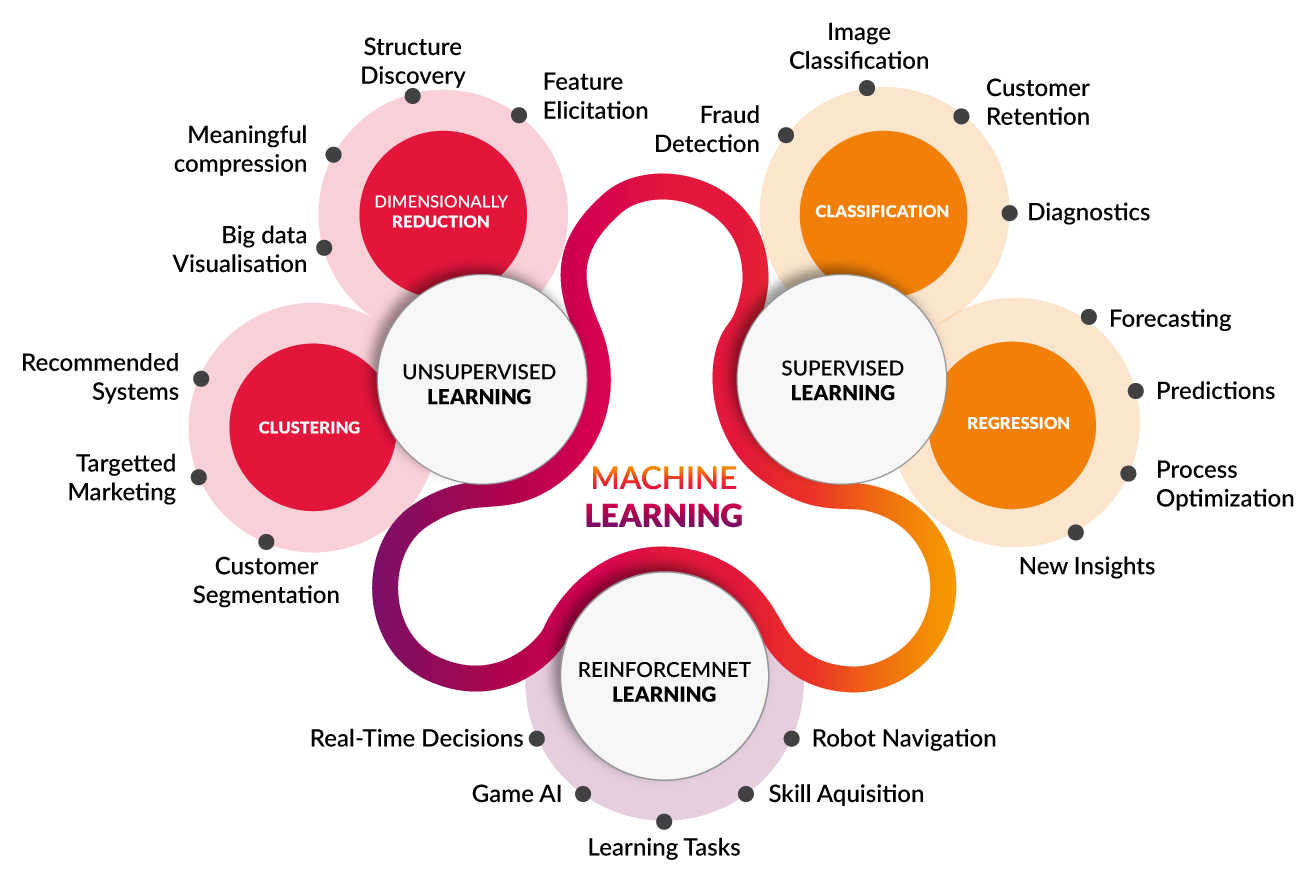
\includegraphics[width=1\linewidth]{media/machine-learning-approaches.png}
    \caption{The three basic learning approaches in machine learning with subcategories and typical applications. The vast majority of machine learning algorithms fall into these three categories.\cite{machine-learning-approaches}}
    \label{fig:machine-learning-approaches}
\end{figure}

Some literature\cite{ml-types1,ml-types2} defines semi-supervised learning, which combines supervised and unsupervised approaches mentioned above, as another learning method. However, since all three basic approaches can be combined, these combinations of learning approaches are omitted in this thesis.

It is also important to mention that the output of a machine learning algorithm, which is usually stored after the learning process and which is subsequently used in the decision-making process, is called a \textbf{model}\cite{algorithms-vs-models}.

\subsection{Supervised learning}

In supervised learning, the program is given a dataset that already contains not only what are the input variables, but also what the correct output should look like. Most times, this dataset is created by a person who knows what the correct output should be - a supervisor. Therefore, this type of learning is called as supervised learning.\cite{all-models}

Supervised learning problems are further categorized into two subcategories, classification and regression problems, depending on what the output is\cite{coursera-ml}. If the output is to be a numerical value, such as the price of a property, it is a regression problem. However, if the output is to be whether or not there is a cat in the picture, then it is classification problem. Also, it can be said that algorithms for regression problems are used to predict continues values and algorithms for classification problems are used to predict (or classify) discrete values.

\subsubsection{Regression}
As mentioned earlier, the output of regression algorithms is continuous values. It can be said that a regression solving algorithm looks for a correlation between the input dependent and independent variables. In detail, the input of the learning algorithm is the first pairs of input dependent and independent variables. The algorithm first searches for the mapping function that best captures the unknown correlation in the learning phase. After that, when the algorithm is presented with data for which we do not know the output, the algorithm uses this learned function to predict the value.

A common example of a regression problem is that a machine learning algorithm predicts property prices based on a dataset of properties sold in the past. This dataset contains features such as a number of rooms, location, property condition, and more. It also contains the sale price. Thus, in the learning phase, the algorithm estimates which features lead to which price. Or rather, what is the correlation between the properties of a property and its selling price. Subsequently, this learned model is saved. Then the algorithm is switched to a mode where it no longer learns but returns the property's price depending on what data it is given.

\subsubsection{Classification}

As with regression, the classification algorithm tries to find the correlation between the dependent and independent variables. The learning and subsequent prediction (classification) also work similarly to regression. The output of classification is not a continuous value but a discrete value. 

For example, it can be a decision whether a cancer is malignant or benign. The number of discrete values can be more than one. Also, the output of the classification does not have to always be a logical true-false value for every classification problem. The classification might recognize whether there is a pig, a dog, or a loaf of bread, or even something more in a picture.

\begin{figure}[ht]
    \centering
    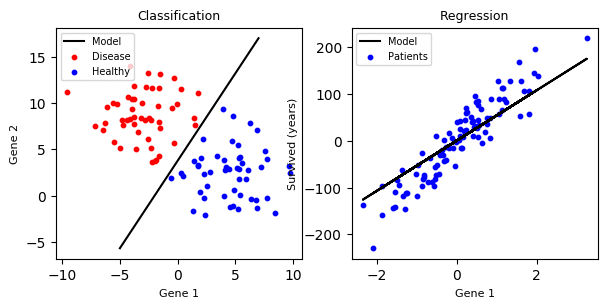
\includegraphics[width=1\linewidth]{media/classification-regression.png}
    \caption{Graph visualization of classification and regression tasks. Classification predicts which set a new patient fits into. Regression predicts the continuous value of the number of years a patient can survive.\cite{classification-regression}}
    \label{fig:classification-regression}
\end{figure}

\subsection{Unsupervised learning}
Unsupervised learning, unlike supervised learning, allows teaching a system without prior knowledge of what the output should look like. This type of learning looks for similarities and patterns in the data instead of mapping input values to labels in the dataset.\cite{coursera-ml}

Unsupervised learning is further divided into two subcategories based on how these similarities and patterns found in the data are used. These subcategories are clustering and dimensional reduction.

\subsubsection{Clustering}

The goal of clustering is to divide data that are similar into groups\cite{ml-types2}. The number of these groups can be an exact number defined by an expert for some algorithms (K-means\cite{k-means}), but there are also algorithms that find the number of groups by themselves (OPTICS\cite{optics}, DBSCAN\cite{dbscan}.

An example of using clustering methods is recommender systems that recommend the same things to users with similar characteristics to other users. Other examples include anomaly detection, statistical data analysis, and social network analysis\cite{clustering-applications}.

Clustering methods are broadly divided into \textbf{hard clustering} and \textbf{soft clustering}, depending on whether individual data points can fall into only one class (hard clustering) or multiple classes (soft clustering). In the case of soft clustering, each data point is scored with a probability measure that determines which clusters the data point belongs to \cite{clustering-types}. 

\textbf{Types of clustering methods:}
\begin{itemize}
    \item Partitioning Clustering
    \item Density-Based Clustering
    \item Hierarchical Clustering
    \item Grid-Based Clustering
    \item Fuzzy Clustering
\end{itemize}

It is not important for this thesis to describe all these types of clustering methods, except the HDBSCAN method (Hierarchical Density-Based Spatial Clustering of Applications with Noise) used in this thesis's practical part. HDBSCAN is a combination of Density-Based Clustering and Hierarchical Clustering. A detailed description and information about the HDBSCAN method are given in Section XY.

\subsubsection{Dimensional reduction}

As mentioned earlier, the main task of dimension reduction algorithms is to transform data from a higher dimensional space to a lower-dimensional space\cite{ml-types2}. This is often done during the preprocessing phase of the data, which can be sparse and contain much redundancy. Dimensional reduction algorithms select the interesting parts of the data in the dataset. This also avoids the problem of the curse of dimensionality\cite{bellman1957dynamic}.

Most dimensionality reduction algorithms are further divided into \textbf{feature extraction} or \textbf{feature elimination} algorithms\cite{ml-types2}.

A very commonly used dimensionality reduction algorithm is Principal component analysis, which is also used in the practical part of this thesis and is described in Chapter XX.

\begin{figure}[ht]
    \centering
    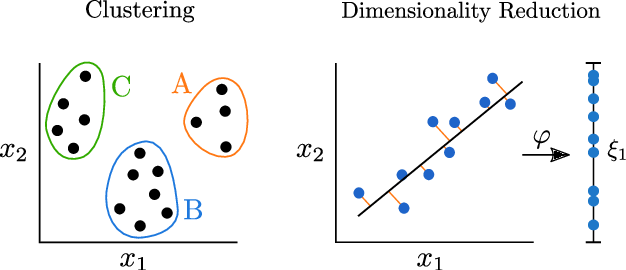
\includegraphics[width=1\linewidth]{media/clustering-reduction.png}
    \caption{Illustration of the output of clustering and dimensional reduction. Clustering searches for patterns among distantly similar data. Dimensional reduction transforms higher dimensional data into lower dimensional data.\cite{clustering-reduction}}
    \label{fig:clustering-reduction}
\end{figure}

